%\documentclass[9pt,twocolumn]{jpc} 

%%%%%%%%%%%%%%%%%%%%%%%%%%%%%%%%%%%%%%%%%%%%%%%%%%%%%%%%%%%%%%%%%%%%%%%%%%%%%%%%%%%%%%%%%%%%%%%%%%%%%%%
%% TODO:
%%%%%%%%%%%%%%%%%%%%%%%%%%%%%%%%%%%%%%%%%%%%%%%%%%%%%%%%%%%%%%%%%%%%%%%%%%%%%%%%%%%%%%%%%%%%%%%%%%%%%%%
%% - Include Sanghyun's information-based Markovity metric?  Include Sanghyun too?
%% - Can we address cases where the eigenvalues of the transition matrix $\mu_k(\tau)$ crash out to near-zero, and explain various trends in the eigenvalues?
%% - Instead of "good" states and "poor" states, perhaps we want to call them something like "decomposition I" and "decomposition II"?
%% - Add back in table comparing estimated free energies of good states estimated from repex, transition matrices, etc.
%%%%%%%%%%%%%%%%%%%%%%%%%%%%%%%%%%%%%%%%%%%%%%%%%%%%%%%%%%%%%%%%%%%%%%%%%%%%%%%%%%%%%%%%%%%%%%%%%%%%%%%

%% Set up PDF/PS automatic figure extension use.
%\newif\ifpdf \ifx\pdfoutput\undefined
%\pdffalse
%\usepackage[dvips]{graphicx}
%\DeclareGraphicsExtensions{.eps,.epsi}
%\else
%\pdfoutput=1
%\pdfcompresslevel=9
%\pdftrue
%\usepackage[pdftex]{graphicx}
%\DeclareGraphicsExtensions{.pdf}
%\fi

%% The figures are in a figures/ subdirectory.
%\graphicspath{{figures/}}

%% Import packages.
%\usepackage{times}                             	% nice fonts
%\usepackage{draftcopy}	            		% DRAFT watermark
%\usepackage{amsmath}                           	% for 'case'
%\usepackage{mathrsfs}                          	% script math font
%\usepackage{url}                               	% allow use of URLs
%\usepackage{latexsym}                           % some math symbols, like \Box

%\newcommand{\T}{\mathrm{T}}                                % T used in matrix transpose
%\newcommand{\tauarrow}{\stackrel{\tau}{\rightarrow}}       % the symbol tau over a right arrow
%\newcommand{\q}{\bfm{q}}
%\newcommand{\p}{\bfm{p}}
%\newcommand{\z}{\bfm{z}}
%\newcommand{\expect}[1]{\langle #1 \rangle}                % <.> for denoting expectations over realizations of an experiment or thermal averages
%\newcommand{\estimator}[1]{\hat{#1}}                       % estimator for some quantity from a finite dataset.
%%\newcommand{\bfm}[1]{\mbox{\boldmath{$#1$}}}               % proper boldface for math environment
%\newcommand{\bfm}[1]{{\bf #1}}
%\newcommand{\program}[1]{\textsc{\lowercase{#1}}}  % Formatting to be used for program or package names.  This uses tiny 

%\setlength{\topmargin}{-1.25in}
%\setlength{\evensidemargin}{-0.25in}
%\setlength{\oddsidemargin}{-0.25in}

%\setlength{\textwidth}{17.8cm}
%\setlength{\textheight}{25.0cm}
%\setlength{\columnsep}{0.8cm}

%\begin{document}

%\title{Describing protein folding kinetics by molecular dynamics simulations. 3. Validation of state space decomposition, with application to terminally-blocked alanine in explicit solvent}

%\author{{\bf John D. Chodera$^1$, William C. Swope$^2$, Jed W. Pitera$^2$, and Ken A. Dill$^3$\thanks{Author to whom correspondence should be addressed: Ken A. Dill {\tt <dill@zimm.compbio.ucsf.edu>}}} \\
%\emph{\normalsize $^1$ Graduate Group in Biophysics and $^3$ Department of Pharmaceutical Chemistry, University of California at San Francisco, San Francisco, CA 94143} \\
%\emph{\normalsize $^2$ IBM Almaden Research Center, 650 Harry Road, San Jose, CA 95120}}

%\maketitle
%\date{}

The material in this chapter is being prepared for submission to \emph{The Journal of Physical Chemistry B} as

\flushleft{\bf Describing protein folding kinetics by molecular dynamics simulations. 3. Validation of state space decomposition, with application to terminally-blocked alanine in explicit solvent}
\flushleft{{\bf John D. Chodera$^1$, William C. Swope$^2$, Jed W. Pitera$^2$, and Ken A. Dill$^3$\thanks{Author to whom correspondence should be addressed: Ken A. Dill {\tt <dill@zimm.compbio.ucsf.edu>}}} \\
\emph{\normalsize $^1$ Graduate Group in Biophysics and $^3$ Department of Pharmaceutical Chemistry, University of California at San Francisco, San Francisco, CA 94143} \\
\emph{\normalsize $^2$ IBM Almaden Research Center, 650 Harry Road, San Jose, CA 95120}}

%%%%%%%%%%%%%%%%%%%%%%%%%%%%%%%%%%%%%%%%%%%%%%%%%%%%%%%%%%%%%%%%%%%%%%%%%%%%%%%%%%%%%%%%%%%%%%%%%%%%%%
% ABSTRACT
%%%%%%%%%%%%%%%%%%%%%%%%%%%%%%%%%%%%%%%%%%%%%%%%%%%%%%%%%%%%%%%%%%%%%%%%%%%%%%%%%%%%%%%%%%%%%%%%%%%%%%
\section*{Abstract}

Despite recent interest in the construction of simple stochastic models to describe the conformational dynamics of peptides and proteins, little work has focused on verifying whether these models provide an accurate description of dynamics.
Previously, we demonstrated that the statistical dynamics of a small solvated peptide (terminally-blocked alanine) over long times could be described by a discrete-state master equation model constructed from short molecular dynamics simulations in explicit solvent \cite{chodera:mms:2006}.  
The accuracy of the model was verified by comparison with a large number of trajectories long enough to reach equilibrium, a method which is impractical for systems with timescales that exceed typical simulation lengths by orders of magnitude.
Here, we focus on how to determine whether a model constructed from short trajectories will accurately reproduce dynamics over long times without the need to conduct additional simulations.
We examine a number of tests of Markovianity to assess their ability determine whether models constructed from these short trajectories will be able to reproduce dynamics over long times, and if so, on what timescale the dynamics appears Markovian.
We use the same solvated peptide system as in a previous work \cite{chodera:mms:2006}, and analyze both good state decompositions (where dynamics is expected to be Markovian on short timescales) and poor decompositions (where dynamics is only Markovian on longer timescales, possibly longer than the short trajectories used to construct the model).

Keywords: master equation model; Markov chain model; molecular dynamics; peptide dynamics; protein folding; transition matrix; rate matrix

%%%%%%%%%%%%%%%%%%%%%%%%%%%%%%%%%%%%%%%%%%%%%%%%%%%%%%%%%%%%%%%%%%%%%%%%%%%%%%%%%%%%%%%%%%%%%%%%%%%%%%
% INTRODUCTION
%%%%%%%%%%%%%%%%%%%%%%%%%%%%%%%%%%%%%%%%%%%%%%%%%%%%%%%%%%%%%%%%%%%%%%%%%%%%%%%%%%%%%%%%%%%%%%%%%%%%%%
\section{Introduction}

Since the first crystallographic studies revealed the intricate three-dimensional structures of proteins, an understanding of the specific mechanisms and general principles governing the process by which they fold has been sought by experimentalists and theorists alike.
Today, fundamental questions, such as whether folding pathways are microscopically homogeneous or heterogeneous, or whether non-native traps or long-lived intermediates exist, remain unresolved.
The ability to characterize folding pathways in detail for even a few proteins would help resolve these questions.
Understanding of folding will also provide insight into the mechanism of protein misfolding diseases, how native structures are encoded by sequence, and how proteins with novel folds and functions might be engineered.

Molecular dynamics simulations allow us to study the folding process in atomic spatial and temporal detail.
However, characterization of protein folding pathways by straightforward molecular dynamics simulation is extremely challenging; proteins fold on the order of microseconds to seconds, while typical molecular simulations reach timescales of only tens of nanoseconds.
In addition, simulations typically model a \emph{single} solvated protein molecule, while experiments generally observe the average behavior of a large \emph{ensemble} of molecules.
While massively parallel supercomputers such as Blue Gene \cite{gara:2005a} can reach timescales of a few microseconds with great feats of engineering \cite{fitch:2003a,germain:2005a}, a useful characterization of a protein folding mechanism would still require a \emph{statistical} description of events.
Such a description could be at a coarse-grained level that fits our level of physical interest, such as ``helix A forms before helix B'' (which we shall term a \emph{pathway} or \emph{route}), with each pathway carrying an associated statistical weight.
If there is more than one pathway, a very large number of folding trajectories would be required to statistically characterize the relative probabilities of different pathways.  
Even if there is only a single folding pathway, our molecular dynamics trajectories would need to be long enough to experience a folding event starting from a suitable unfolded state, and a sufficient number of trajectories would need to be collected to establish that there is only a single pathway.
Distributed computing projects now allow for the collection of thousands of trajectories tens of nanoseconds in length, such that a small number of them can contain folding events \cite{pande:2000a,zagrovic:2002a}.
Unfortunately, the possibility remains that folding events observed in short trajectories may be statistically different from the bulk of folding events, which occur over much longer timescales \cite{fersht:2002a,marianayagam:2005a}.  

In order to statistically characterize probable folding routes or verify that only single routes dominate, it is necessary to construct a model from which these probabilities can be computed using simulation data that can be obtained with reasonable computational effort.  
Master equation or Markov chain models \cite{vankampen,swope:2004a,singhal:2004a,chodera:mms:2006} present such a solution.
Master equations are Markov models of dynamics either in the low dimensional manifold of the slow degrees of freedom or, as we consider here, a discrete state space where the states correspond to approximations of the metastable conformational substates accessible to the molecule.  
These models can describe dynamics either in discrete time (here termed a \emph{Markov chain model}) or in continuous time (\emph{master equation model}); in either case it is understood that there is a coarse-graining of the time coordinate such that only processes occurring slower than a given timescale are adequately described by the given model.
Once the model is constructed and the timescale for Markovian behavior determined, it can be used to compute the stochastic temporal evolution of either a single macromolecule or a population of noninteracting macromolecules, allowing direct comparison of simulated and experimental observables for both single-molecule or ensemble kinetics experiments.
In addition, useful properties difficult to access experimentally, such as state lifetimes \cite{swope:2004a}, relaxation from experimentally inaccessible prepared states \cite{chodera:mms:2006}, mean first-passage times \cite{singhal:2004a}, the existence of hidden intermediates \cite{ozkan:2002a}, and $P_\mathrm{fold}$ values \cite{lenz:2004a} or committor distributions \cite{geissler:jpcb:1999}, can easily be obtained.

Such models are a natural choice for representing protein dynamics, in which processes with intrinsic timescales ranging from femtoseconds (\emph{e.g.}\ bond vibrations) to microseconds or milliseconds (folding) can be identified. 
If there is a clear \emph{separation of timescales} between fast, uninteresting dynamics and slow, large-scale conformational changes, then these models can provide an excellent description of the slow dynamics of interest.
% JDC: Something about diffusive dynamics as well?
Several groups have demonstrated that the hierarchical nature of the energy landscape results in a natural separation of timescales in peptide simulations with implicit models of solvent \emph{in vacuo} \cite{levy:2001a, mortenson:2001a}, a property that may also hold for solvated systems.
% JDC: Need more refs here?

Construction of master equation models for realistic molecular mechanics systems has, however, proved problematic. 
Techniques based on enumerating all minima and computing interstate transition rates with transition state theory have proved insightful for simple systems \emph{in vacuo} or with an implicit model of solvent \cite{czerminski:1990a,kunz:1995a,ball:1998b,levy:2001a,mortenson:2001a,mortenson:2002a,evans:2004a}, but as the number of minima grows exponentially with system size, this procedure rapidly becomes untenable for larger proteins or systems containing explicit solvent.
Due to these limitations, much work has focused on the construction of discrete- or continuous-time Markov models to describe dynamics among a small number of states which may each contain many minima within large regions of configuration space \cite{grubmueller:1994a,degroot:2001a,swope:2004b,singhal:2004a,levy:2005a,sorin:2005b,sriraman:2005a,schultheis:2005a,singhal:2005a,elmer:2005b,park:2006a}.

Here, we follow a method for the construction of a discrete-state master equation model based on calculation of state-to-state time-correlation functions proposed by Swope \emph{et al.}\ \cite{swope:2004a}.  
A previous investigation applying this method to a model system (terminally-blocked alanine peptide in explicit solvent) demonstrated that a 6-state Markov chain model with a time resolution of 6 ps constructed from short (10 ps) trajectories was able to describe dynamics over timescales of at least 100 ps \cite{chodera:mms:2006}.
In that work, accurate reproduction of statistical dynamics was verified by comparison with a separate set of long (100 ps) trajectories.
%The utility of a Markov model would be lost if simulation of a large number of trajectories as long as the process of interest was necessary in order to validate the model.
The goal, however, is to construct and validate models of dynamics to allow long timescales to be reached without the need to generate long trajectories.
A method is needed to determine the timescale at which the model will be Markovian and decide between multiple state decompositions given only the set of short trajectories used to construct the model.

% JDC: Revise this to emphasize validation
Here, we focus on how to determine whether a particular choice of state definitions can lead to a master equation model capable of adequately describing interstate dynamics and for what coarse-grained timescale this model will be accurate.
Since the optimal state definition must generally be arrived at through trial and error, we perform several tests to discriminate among alternate choices of state definitions to determine which choice results in the most \emph{useful} master equation model.
We consider terminally-blocked alanine peptide in explicit solvent as a model system where the slow degrees of freedom, the $(\phi, \psi)$ torsions, are known \emph{a priori}.  
Since there are only two slow degrees of freedom\footnote{Simulations of alanine dipeptide examining the committor distribution have implicated solvent coordinates as the next-slowest degrees of freedom \cite{bolhuis:2000a,ma:2005a}, but we have previously verified that $\phi$ and $\psi$ torsions form a sufficient basis for the slow degrees of freedom on timescales of 6 ps and greater \cite{chodera:mms:2006}.}, we construct a two-dimensional potential of mean force (PMF) in these coordinates by simulation, and visually identify the metastable conformational substates.
In this way, we can separate the problem of finding a good decomposition into metastable states from that of computing transition rates and assessing the resulting master equation model.  

As in Ref.\ \cite{swope:2004a}, we first obtain a broad sampling of conformation space by way of a parallel tempering simulation, from which we also obtain the PMF and from this, the state decomposition.
A number of short trajectories are then initiated from an equilibrium distribution within each state obtained from the parallel tempering simulation in order to collect state-to-state transitions.  
These simulations can then be used to construct an interstate transition matrix and determine the timescale for which the underlying rate matrix becomes an adequate description of the dynamics.

This paper is organized as follows:
In Section \ref{validation:section:theory}, we briefly review the the discrete-state master equation and Markov chain theory and the basic concepts behind its construction from simulation data.  
Section \ref{validation:section:application-to-alanine-dipeptide} introduces the terminally-blocked alanine in explicit solvent model system (the same system considered in a previous study \cite{chodera:mms:2006}) that will be used to assess the utility of various tests of Markovianity.
Finally, Section \ref{validation:section:validation} describes a number of such tests and their observed performance in determining the time for the emergence of Markovian behavior for this model system.

%%%%%%%%%%%%%%%%%%%%%%%%%%%%%%%%%%%%%%%%%%%%%%%%%%%%%%%%%%%%%%%%%%%%%%%%%%%%%%%%%%%%%%%%%%%%%%%%%%%%%%
% THEORY
%%%%%%%%%%%%%%%%%%%%%%%%%%%%%%%%%%%%%%%%%%%%%%%%%%%%%%%%%%%%%%%%%%%%%%%%%%%%%%%%%%%%%%%%%%%%%%%%%%%%%%
\section{Master equation and Markov models}
\label{validation:section:theory}

\subsection{The discrete-state master equation.}
\label{validation:section:master-equation-review}

The dynamical evolution of a discrete-state, continuous-time process that is Markovian on all timescales is governed by the so-called \emph{master equation} (see, for example, van Kampen \cite{vankampen} for an excellent review) which can be written as
\begin{equation}
\frac{\partial}{\partial t} \bfm{p}(t) = \bfm{K} \bfm{p}(t) . \label{validation:equation:master-equation}
\end{equation}
Here, $\bfm{p}(t) \in \Re^M$, where $p_i(t)$ denotes the probability of state $i$ being occupied at time $t$, requiring $p_i \ge 0$ and $\sum_{i=1}^M p_i = 1$.  
$\bfm{K}$ is the matrix of rate constants, with $K_{ji}$ denoting the rate constant associated with the transition from state $i$ to state $j$ if $j \ne i$, and the diagonal elements determined such that the columns sum to zero to ensure conservation of total probability, {\emph i.e.}, $K_{ii} = - \sum_{j \ne i}^M K_{ji}$.  
The equilibrium (or \emph{stationary}) distribution $\bfm{p}_\mathrm{eq}$ is given by
\begin{equation}
\frac{\partial}{\partial t} \bfm{p}_\mathrm{eq} = \bfm{K} \bfm{p}_\mathrm{eq} = \bfm{0} .
\end{equation}
For the systems we consider here, we shall presume that only one stationary distribution exists.

In problems of physical interest, the rate matrix $\bfm{K}$ statisfies the condition of $\emph{detailed balance}$
\begin{equation}
K_{ji} \, p_{\mathrm{eq},i}  = K_{ij} \, p_{\mathrm{eq},j} .
\end{equation}
As a result, $\bfm{K}$ is related to a symmetric matrix $\tilde{\bfm{K}}$ by a similarity transformation
\begin{eqnarray}
\tilde{\bfm{K}} = \bfm{D}^{-{1/2}} \bfm{K} \bfm{D}^{{1/2}} = \bfm{D}^{{1/2}} \bfm{K}^\T \bfm{D}^{-{1/2}} = \tilde{\bfm{K}}^\T
\end{eqnarray}
where $\bfm{D} = \mathrm{diag}( \bfm{p}_\mathrm{eq})$ is the diagonal matrix of equilibrium probabilities.  $\tilde{\bfm{K}}$ is therefore orthogonally diagonalizable
\begin{equation}
\tilde{\bfm{K}} = \tilde{\bfm{U}} \tilde{\bfm{\Lambda}} \tilde{\bfm{U}}^\mathrm{T}
\end{equation}
with $\tilde{\bfm{U}} \tilde{\bfm{U}}^\mathrm{T} = \bfm{I}$ and $\tilde{\bfm{\Lambda}} = \mathrm{diag}(\tilde{\lambda_1}, \tilde{\lambda_2}, \ldots, \tilde{\lambda_M})$ is the diagonal matrix of eigenvalues, sorted such that $\lambda_1 \ge \lambda_2 \ge \cdots \ge \lambda_M$.  
$\bfm{K}$ shares the same eigenvalues as $\tilde{\bfm{K}}$:
\begin{equation}
\bfm{K} = \bfm{D}^{1/2} \tilde{\bfm{K}} \bfm{D}^{-{1/2}} = \left( \bfm{D}^{1/2} \tilde{\bfm{U}} \right) \tilde{\bfm{\Lambda}} \left( \bfm{D}^{1/2} \tilde{\bfm{U}} \right)^{-1} = \bfm{U} \bfm{\Lambda} \bfm{U}^{-1}
\end{equation}
but the eigenvectors differ by a factor of $\bfm{D}^{1/2}$.
All the eigenvalues are real, and exactly one eigenvalue, $\lambda_1$, is zero --- all others are negative.

The time evolution of an initial probability vector $\bfm{p}(0)$ is given by the solution to Eq.\ \ref{validation:equation:master-equation}
\begin{equation}
\bfm{p}(t) = e^{\bfm{K} t} \bfm{p}(0) \equiv \bfm{T}(t) \bfm{p}(0) \label{validation:equation:master-equation-time-evolution}
\end{equation}
where $e^{\bfm{K} t}$ denotes the matrix exponential, and $\bfm{T}(t)$ is called the \emph{transition matrix}, as element $T_{ji}(t)$ denotes the probability of observing the system in state $j$ a time $t$ after initially observing it in state $i$\footnote{We adopt the notation of a \emph{column-stochastic} transition matrix, where the columns of $\bfm{T}(t)$ sum to unity. In mathematical literature on Markov chains, and in some publications cited here, it is often common to instead see \emph{row-stochastic} transition matrices, where the rows sum to unity, and evolution is governed by the equation $[\bfm{p}(t)]^\T = [\bfm{p}(0)]^\T \bfm{T}(t)$}.
$\bfm{T}(\tau)$ is sometimes also referred to as the \emph{propagator}, as its operation on a probability vector $\bfm{p}(t)$ evolves the distribution by a fixed time $\tau$.  
The eigenvalues of $\bfm{T}(t)$ and $\bfm{K}$ are simply related
\begin{equation}
\bfm{T}(t) = \bfm{U} \bfm{M} \bfm{U}^{-1} = e^{\bfm{K} t} = \bfm{U} e^{\bfm{\Lambda} t} \bfm{U}^{-1} \label{validation:equation:relation-between-eigenvalues-of-transition-and-rate-matrix}
\end{equation}
where $\bfm{M} = \mathrm{diag}(\mu_1, \mu_2, \ldots, \mu_M)$ is the matrix of eigenvalues of the transition matrix, which lie in the interval $[0,1]$.
Because $\bfm{U} = \bfm{D}^{1/2} \tilde{\bfm{U}}$, this decomposition allows us to write $\bfm{T}(t)$ as an expansion over the eigenvectors of $\tilde{\bfm{K}}$ as
\begin{equation}
\bfm{T}(t) = \sum_{k=1}^M \bfm{D}^{{1/2}} \, \tilde{\bfm{u}}_k \, e^{\lambda_k t} \, \tilde{\bfm{u}}_k^\T \, \bfm{D}^{-{1/2}} . \label{validation:equation:eigenvector-expansion-of-transition-matrix}
\end{equation}

For physical systems, we do not expect Eq. \ref{validation:equation:master-equation-time-evolution} to hold for all times once we have coarse-grained space into states.
Instead, the rates $K_{ji}$ reflect \emph{phenomenological rates} that may only correctly describe interstate transitions after some coarse-grained \emph{internal equilibration time} $\tau_{\mathrm{int}}$ \cite{chandler:1978a}.
Because of this, states that do not share a boundary in configuration space may still have nonzero phenomenological transition rates connecting them \cite{voter:1985a}.
Additionally, for physical systems in which all states are accessible, there is always some probability that a system prepared in one state will have a momentum that will carry it to another state some finite time $\tau$ later, so that all transition elements $T_{ji}(\tau)$ should be nonzero, though they may be very small.

\subsection{Construction from molecular dynamics simulation.}
\label{validation:section:construction-from-simulation}

Here, we briefly review the construction of a discrete-state master equation model from simulation.  
We obtain the same expressions as in Ref.\ \cite{swope:2004a}, but our exposition and notation differs slightly.

We denote a point in phase space by $\bfm{z} = (\bfm{q}, \bfm{p})$, where $\bfm{q},\bfm{p} \in \Re^{3N}$ are the coordinates and momenta, respectively.  
A trajectory in phase space of time length $T$ is denoted $\bfm{z}(t), \, t \in [0,T]$, with $t$ denoting the time index.  
The system has Hamiltonian 
\begin{equation}
H(\bfm{z}) = \frac{1}{2} \bfm{p}^{\T} \bfm{M}^{-1} \bfm{p} + V(\bfm{q})
\end{equation}
where $\bfm{M}$ is the diagonal matrix of atomic masses, and $V(\bfm{q})$ is the potential function.  
The equilibrium average of a phase function or mechanical observable $A(\bfm{z})$ is given by the expectation over the canonical ensemble
\begin{equation}
\left< A \right> = \frac{\int d\bfm{z} \, e^{-\beta H(\bfm{z})} \, A(\bfm{z})}{\int d\bfm{z} \, e^{-\beta H(\bfm{z})} }
\end{equation}
where $\beta = (k_B T)^{-1}$ denotes the inverse temperature.
Similarly, the average over a functional of trajectories $A[\bfm{z}(t)]$, which depends on the value of $\bfm{z}(t)$ at multiple times, is given by
\begin{equation}
\left< A[\bfm{z}(t)] \right> \equiv \frac{\int \mathcal{D}[\bfm{z}(t)] \, \mathcal{P}[\bfm{z}(t)] \, A[\bfm{z}(t)]}{\int \mathcal{D}[\bfm{z}(t)] \, \mathcal{P}[\bfm{z}(t)]} \
\end{equation}
where $\mathcal{D}[\bfm{z}(t)]$ is the differential over constant-energy trajectories $\bfm{z}(t)$ and $\mathcal{P}[\bfm{z}(t)]$ is the probability density of paths.
We presume dynamics is governed by Hamilton's equations of motion\footnote{In this study and the previous one \cite{chodera:mms:2006}, we employ dynamical simulations with bond length constraints for efficiency purposes.  Technically, this causes dynamics to be non-Hamiltonian \cite{fixman:1974a,tuckerman:2001a}, but we assume this difference is unimportant for the purposes of our analyses.  In future, multiple timestep integrators (\emph{e.g.}\ \cite{tuckerman:1992a}) could be used to void loss in efficiency while eliminating the need for bond length constraints.}
\begin{equation}
\frac{\partial}{\partial t}\bfm{q} = \nabla_{\bfm{p}} H \; ; \: \frac{\partial}{\partial t}\bfm{p} = - \nabla_{\bfm{q}} H . \nonumber
\end{equation}
which allows us to rewrite the expectation over functionals of trajectories as
\begin{equation}
\left< A[\bfm{z}(t)] \right> = \frac{\int d\bfm{z}(0) \, e^{-\beta H(\bfm{z}(0))} \, A[\bfm{z}(t)]}{\int d\bfm{z} \, e^{-\beta H(\bfm{z})}} .
\end{equation}

We suppose that we have already followed some procedure to generate a decomposition of phase space into a complete set of $M$ non-overlapping regions $\mathcal{S}_i$, which we term \emph{states}, that together form a complete covering of phase space.  
We define an \emph{indicator function} $\chi_i(\bfm{z})$ for state $i$ such that
\begin{eqnarray}
\chi_i(\bfm{z}) = 
\begin{cases}
1 & \mathrm{if} \, \bfm{z} \in \mathcal{S}_i \nonumber \\
0 & \mathrm{otherwise.}
\end{cases}
\end{eqnarray}
Since the states form a complete covering of phase space, we have
\begin{eqnarray}
\sum_{i=1}^M \chi_i(\bfm{z}) = 1 \: \forall \: \bfm{z} . \nonumber
\end{eqnarray}
Furthermore, we presume these states are only functions of configuration $\bfm{q}$, that is, $\chi_i(\bfm{z}) = \chi_i(\bfm{q})$.

As the phenomenological transition rates $K_{ji}$ are not directly observable, and may not even exist at short times, our procedure instead involves computing the observed state-to-state transition probabilities $T_{ji}(\tau)$ \cite{swope:2004a}.
We shall often refer to the evolution time $\tau$ as the \emph{lag time} because it refers to the time between subsequent observations of the system. 
Formally, this transition probability is defined as
\begin{eqnarray}
T_{ji}(\tau) &\equiv& \frac{C_{ji}(\tau)}{\sum\limits_{j'=1}^M C_{j'i}(\tau)} = \frac{C_{ji}(\tau)}{p_{\mathrm{eq},i}} \label{validation:equation:transition-probabilities}
\end{eqnarray}
where we have defined the state-state time correlation function $C_{ji}(\tau)$ by
\begin{eqnarray}
C_{ji}(\tau) &\equiv& \left< \chi_j(\bfm{z}(\tau)) \, \chi_i(\bfm{z}(0)) \right> \\
&=& \left< \chi_i(\bfm{z}(0)) \, \chi_j(\bfm{z}(\tau)) \right> \nonumber \\
&=& C_{ij}(\tau) \nonumber .
\end{eqnarray}
The second equality follows by time-reversal symmetry of Newtonian trajectories and the invariance of the $\chi_i(\bfm{z})$ to inversion of the momenta.

%%%%%%%%%%%%%%%%%%%%%%%%%%%%%%%%%%%%%%%%%%%%%%%%%%%%%%%%%%%%%%%%%%%%%%%%%%%%%%%%%%%%%%%%%%%%%%%%%%%%%%
% APPLICATION TO ALANINE DIPEPTIDE
%%%%%%%%%%%%%%%%%%%%%%%%%%%%%%%%%%%%%%%%%%%%%%%%%%%%%%%%%%%%%%%%%%%%%%%%%%%%%%%%%%%%%%%%%%%%%%%%%%%%%%
\section{Terminally-blocked alanine peptide in explicit solvent as a model system}
\label{validation:section:application-to-alanine-dipeptide}

Here, we describe the terminally-blocked alanine in explicit solvent model system considered in this study to evaluate various tests of Markovianity.
Previously, it was determined that a Markov chain model constructed for this system using a lag time of 6 ps was able to describe the statistical dynamical evolution over long times, as verified by an independent set of 100 ps trajectories \cite{chodera:mms:2006}.
For convenience, we describe the protocol used here to generate the simulation data (the same data as considered in Ref.\ \cite{chodera:mms:2006}) and the methods used to estimate transition probabilities.

\subsection{System setup and equilibration.}
\label{validation:section:system-setup-and-equilibration}

Using the \program{LEaP} program from the \program{AMBER7} molecular mechanics package \cite{AMBER7}, a terminally-blocked alanine peptide (sequence Ace-Ala-Nme, see Figure \ref{validation:figure:2d-pmf}) was generated in the extended conformation and subsequently solvated with 431 TIP3P water molecules \cite{jorgensen:1983a} in a truncated octahedral simulation box whose dimensions were chosen to ensure a minimum of $7$ \AA\ distance from the peptide to the box faces.  
Peptide force field parameters were taken from the AMBER parm96 parameter set \cite{AMBER-parm96}.  
All molecular dynamics simulations were conducted using the {\tt sander} program from the \program{AMBER7} package.  
Default nonbonded cutoffs were used, bonds to hydrogen were constrained with SHAKE using a tolerance of $10^{-8}$ \AA\ \cite{SHAKE}, and long-range electrostatics were treated by the particle-mesh Ewald (PME) method \cite{darden:1993a} with the default settings.

The system was first subjected to 50 steps of steepest descent energy minimization, followed by 1000 steps of conjugate gradient optimization.
To equilibrate the explicit solvent system to the appropriate volume, a 100 ps molecular dynamics simulation was performed with the temperature adjusted to 300 K and the pressure to 1 atm by the Berendsen weak-coupling algorithm \cite{berendsen:1984a} with temperature and pressure relaxation time constants of 1 ps and 0.2 ps, respectively.
The simulation box was fixed at the final size obtained from this equilibration step, with a volume of 13 232 \AA$^3$, in all subsequent simulations.

\subsection{Parallel tempering simulation.}
\label{validation:section:parallel-tempering}

In order to broadly explore the configuration space of the peptide and ensure that all important conformational substates were located, a parallel tempering (also known as replica-exchange among temperatures) molecular dynamics simulation \cite{sugita:1999a} was conducted using a parallel {\tt Perl} wrapper for the {\tt sander} program\footnote{A copy of this Perl wrapper to perform replica-exchange simulations using AMBER7 and AMBER8 can be obtained from \url{http://www.dillgroup.ucsf.edu/~jchodera/code/rex}.}.
Forty replicas were used, with replica temperatures exponentially distributed over the range 273--600 K, yielding an average exchange acceptance probability of about 50\%.
All momenta were reassigned from the Maxwell-Boltzmann distribution at the appropriate replica temperature after each exchange attempt, and constant-energy, constant-volume molecular dynamics with a 2 fs timestep was performed between exchange attempts.
The algorithm used to select pairs of replicas for temperature exchange attempts starts from the highest-temperature replica and attempts to swap the configuration for the next-lowest temperature replica using the Metropolis-like criteria, and proceeds down the temperatures in this manner.  On the next iteration, swapping attempts start from the lowest temperature and proceed upward, and this alternation in direction is continued in subsequent pairs of iterations.

Starting all replicas from the 300 K NPT-equilibrated configuration described above, 100 iterations were conducted with 1 ps between exchange attempts to equilibrate the replicas to their respective temperatures.  
This equilibration run was followed by a production run of 500 iterations with 20 ps between exchange attempts, producing a total of 10 ns/replica, or 400 ns in aggregate, for the production run. 
The longer time between exchanges for the production run was chosen so as not to hinder transitions by frequent velocity randomization.  
Solute snapshots and potential energies were stored during the production run every 0.1 ps for the purposes of estimating the free energies of each state (resulting in $4\cdot10^6$ saved solute configurations), and full-system restart files were saved every 1 ps (yielding $4\cdot10^5$ restart files) for the purpose of starting shooting simulations from these configurations, described below in Section \ref{validation:section:shooting-simulations}.

%\subsection{State decomposition.}
%\label{validation:section:state-decomposition}

%The slow degrees of freedom for terminally-blocked alanine peptide (neglecting those involving solvent motion) can be captured by the two backbone torsion angles labeled $\phi$ and $\psi$ (see Figure \ref{validation:figure:2d-pmf}) \cite{bolhuis:2000a,ma:2005a}. To this end, the potential of mean force at 302 K was computed from the parallel tempering data using the weighted histogram analysis method (WHAM) \cite{kumar:1992a,chodera:2006a} and is shown in Figure \ref{validation:figure:2d-pmf}.  Six free energy basins are readily visible, and rectangular regions around these basins were chosen for the decomposition of all of configuration space into a set of six states.  State definitions are listed in Table \ref{validation:table:state-definitions} and plotted as thick dividing lines in Figure \ref{validation:figure:2d-pmf}.

\subsection{State decomposition.}
\label{validation:section:state-decomposition}

In more complex molecular systems, it is generally a difficult problem to identify the ``slow'' degrees of freedom involved in conformational transitions between metastable states.  
Here, we postulate that only a subset of the solute degrees of freedom will be necessary to accurately describe the long-time dynamics of the system.  
We presume the solvent will be important in determining the inter-state rate constants, but plays no real role in determining the gross structure of the conformational substates at long timescales.  
To this end, the potential of mean force of the two backbone torsion angles $\phi$ and $\psi$ at 302 K was estimated from the parallel tempering data using the weighted histogram analysis method (WHAM) \cite{kumar:1992a,chodera:jctc:2006} and is shown in Figure \ref{validation:figure:2d-pmf}.  
Six free energy basins are readily visible, and rectangular regions around these basins were manually chosen as previously \cite{chodera:mms:2006} to serve as a ``good'' decomposition of all of configuration space into a set of six states for the construction of a discrete-state master equation model.
These states are depicted in Figure \ref{validation:figure:2d-pmf}, alongside a ``poor'' 6-state decomposition, in which the boundaries have been significantly displaced so as to include internal barriers within states\footnote{The poor partitioning was defined as follows: (1) $\phi \in [(179,-135]$, $\psi \in (98,48]$; (2) $\phi \in (-135,-60]$, $\psi \in (98,48]$; (3) $\phi \in (179,-135]$, $\psi \in (48,98]$; (4) $\phi \in (-135,-60]$, $\psi \in (48,98]$; (5) $\phi \in (-60,179]$, $\psi \in (98,-45]$; (6) $\phi \in (-60,179]$, $\psi \in (-45,98]$.  Specified intervals denote intervals on the torus, which is continuous from -180 to +180.  All torsion angles are specified in degrees.}.
Two additional state decompositions were considered, both of which were ``lumpings'' of the good 6-state decomposition.
A ``good'' lumping, which is intended to be minimally perturbative on the long timescales, was constructed by lumping states 1 and 2, as well as states 3 and 4, as each pair of states is only separated by low free energy barriers.
A ``poor'' lumping was also constructed by lumping states 1, 4, and 5 together into a single state containing large internal barriers, which is expected to disrupt the ability to produce a good model of the statistical dynamics from short simulations.

%Relative free energies at 302 K of states from the good decomposition estimated from the parallel tempering simulation by WHAM are shown in Table \ref{validation:table:state-free-energies}.
%Note that states 5 and 6 are rather high in free energy, necessitating the use of parallel tempering and reweighting techniques in order to sample them adequately.

It should be noted that this approach to state decomposition is only reasonable if the PMF in the complete set of slow degrees of freedom can be computed and examined --- projection onto an arbitrary set of structural observables or order parameters (such as the number of native contacts and radius of gyration) and identification of basins as metastable states is not the same thing.  When arbitrary order parameters are used, there is no guarantee that connected regions in the low-dimensional order parameter space correspond to single, connected regions in phase space, a requirement for a Markovian model of dynamics.
Additionally, the projection must account for the Jacobian, so as not to distort space so much that free energy barriers are not artificially introduced or eliminated \cite{hartmann:2004a,hartmann:2004b}.

\begin{figure}[tbp]
  \begin{center}
%    \resizebox{3.375in}{!}{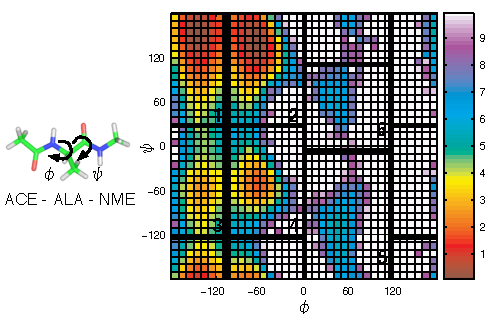
\includegraphics{figures/2d_pmf.pdf}}
    \resizebox{3.375in}{!}{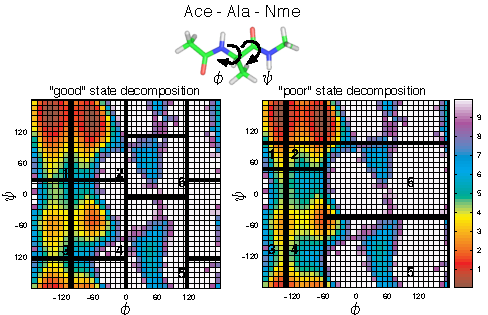
\includegraphics{chapters/mastereqn-alanine-validation/figures/2d-pmf-good-and-bad-states.pdf}}
  \end{center}
  \caption{
  {\bf Terminally-blocked alanine and potential of mean force at 302 K.}  
  Top: The terminally-blocked alanine peptide with $(\phi,\psi)$ torsions labeled.  
  Bottom: The potential of mean force in the $(\phi,\psi)$ torsions at 302 K estimated from the parallel tempering simulation, with ``good'' (left) and ``poor'' (right) state decompositions labeled, and colorbar graded in units of $k_B T$ and truncated at $10 k_B T$ (white).  
  }
  \label{validation:figure:2d-pmf}
\end{figure}

% JDC: Change this into a table that shows: state # ; good states phi/psi ; bad states phi/psi
%\begin{table}[tbp]
%\caption{{\bf State definitions for the manual decomposition of $(\phi,\psi)$-space into metastable states and populations at 302 K.}}
%\label{validation:table:state-definitions}
%\begin{center}
%\begin{tabular}{ccccc}
%\hline 
%      &                        & \multicolumn{2}{c}{state definitions} & \\
%\cline{3-4}
%state & label$^a$ & $\phi$ & $\psi$ & population$^b$ \\
%\hline
%1 & $\mathrm{C}_5$             & $[117, \, -105)$ & $[28, \, -124)$ & .4787 (.0613) \\
%2 & $\mathrm{P}_\mathrm{II}$   & $[-105, \, 0)$   & $[28, \, -124)$ & .4159 (.0486) \\
%3 & $\alpha_\mathrm{P}$        & $[117, \, -105)$ & $[-124, \, 28)$ & .0425 (.0038) \\
%4 & $\alpha_\mathrm{R}$        & $[-105, \, 0)$   & $[-124, \, 28)$ & .0588 (.0079) \\
%5 & $\mathrm{C}_7^\mathrm{ax}$ & $[0, \, 117)$    & $[111, \, -5)$  & .0030 (.0015) \\
%6 & $\alpha_\mathrm{L}$        & $[0, \, 117)$    & $[-5, \, 111)$  & .0011 (.0004) \\
%\end{tabular}
%\end{center}
%\par\medskip\footnotesize
%$^a$ Corresponding state labels from \cite{roterman:1989a}.  $^b$ Population estimate at 302 K from replica exchange simulation and WHAM.
%\end{table}

%\begin{table*}[tbp]
%\caption{{\bf Estimated state free energies and uncertainties at 302 K for good state decomposition from parallel tempering, shooting simulations, and transition matrices, in kcal/mol.}}
%\label{validation:table:state-free-energies}
%\begin{center}
%\begin{tabular}{ccccccccccc}
%\hline 
%      &       & \multicolumn{4}{c}{100 ps shooting trajectories} && \multicolumn{4}{c}{10 ps shooting trajectories} \\
%\cline{3-6} \cline{8-11}
%state & repex$^a$ & avg$^b$ & $\bfm{T}$(0.1 ps)$^c$ & $\bfm{T}$(1 ps)$^c$ & $\bfm{T}$(10 ps)$^c$ && avg$^b$ & $\bfm{T}$(0.1 ps)$^c$ & $\bfm{T}$(1 ps)$^c$ & $\bfm{T}$(10 ps)$^c$ \\
%\hline
%1 & $0.00 \, (.08)$ & $0.00 \, (.00)$ & $0.00 \, (.00)$ & $0.00 \, (.00)$ & $0.00 \, (.00)$ && $0.00 \, (.00)$ & $0.00 \, (.00)$ & $0.00 \, (.00)$ & $0.00 \, (.00)$ \\
%2 & $0.08 \, (.07)$ & $0.11 \, (.00)$ & $0.11 \, (.00)$ & $0.11 \, (.00)$ & $0.11 \, (.00)$ && $0.00 \, (.00)$ & $0.00 \, (.00)$ & $0.00 \, (.00)$ & $0.00 \, (.00)$ \\
%3 & $1.15 \, (.05)$ & $1.46 \, (.00)$ & $1.46 \, (.00)$ & $1.46 \, (.00)$ & $1.46 \, (.00)$ && $0.00 \, (.00)$ & $0.00 \, (.00)$ & $0.00 \, (.00)$ & $0.00 \, (.00)$ \\
%4 & $1.26 \, (.08)$ & $1.27 \, (.00)$ & $1.27 \, (.00)$ & $1.27 \, (.00)$ & $1.27 \, (.00)$ && $0.00 \, (.00)$ & $0.00 \, (.00)$ & $0.00 \, (.00)$ & $0.00 \, (.00)$ \\
%5 & $3.05 \, (.30)$ & $3.08 \, (.00)$ & $3.28 \, (.00)$ & $3.28 \, (.00)$ & $3.29 \, (.00)$ && $0.00 \, (.00)$ & $0.00 \, (.00)$ & $0.00 \, (.00)$ & $0.00 \, (.00)$ \\
%6 & $3.66 \, (.23)$ & $3.73 \, (.00)$ & $3.73 \, (.00)$ & $3.73 \, (.00)$ & $3.75 \, (.00)$ && $0.00 \, (.00)$ & $0.00 \, (.00)$ & $0.00 \, (.00)$ & $0.00 \, (.00)$ \\
%\end{tabular}
%\end{center}
%\par\medskip\footnotesize
%$^a$ Replica-exchange simulation.  $^b$ Average over all snapshots of shooting trajectories, weighted by probability of occupying initial state obtained from replica-exchange simulation.  $^c$ Obtained from equilibrium eigenvector of the transition matrix.
%\end{table*}

\subsection{Shooting simulations.}
\label{validation:section:shooting-simulations}

In order to construct a discrete-state master equation model once the states have been identified, we must obtain reliable estimates of the interstate transition probabilities. 
While a number of equilibrium trajectories could be used for this purpose, states of high free energy would be visited only infrequently, resulting in the transition elements of these states being poorly determined.
Swope \emph{et al.}\ proposed the use of \emph{selection cells}, (potentially overlapping) regions which together form a complete covering of configuration space from which sets of trajectories are initiated \cite{swope:2004a}.
The purpose of these selection cells is to allow more trajectories from high free energy regions to be harvested, allowing the transition matrix to be determined to sufficient precision.

Here, we choose to initiate sets of trajectories from a set of selection cells that are coincident with the six states of the ``good'' manual decomposition described above.
For this case, we may decompose the expectation of any property that is a functional of trajectories, $\expect{A[\z(t)]}$, into a weighted sum over conditional expectations:
\begin{eqnarray}
\lefteqn{\expect{A[\z(t)]} = \frac{\int d\z(0) \, e^{-\beta H(\z(0))} \, A[\z(t)]}{\int d\z \, e^{-\beta H(\z)}}} \nonumber \\
&=& \frac{\int d\z(0) \, \left[ \sum\limits_{i=1}^M \chi_i(\z(0)) \right] \, e^{-\beta H(\z(0))} \, A[\z(t)]}{\int d\z \, \left[ \sum\limits_{i=1}^M \chi_i(\z(0)) \right] \, e^{-\beta H(\z)}} \nonumber \\
&=& \frac{\sum\limits_{i=1}^M \left[ \frac{\int d\z \, \chi_i(\z) \, e^{-\beta H(\z)}}{\int d\z \, e^{-\beta H(\z)}} \right] \left[ \frac{\int d\z(0) \, \chi_i(\z(0)) \, e^{-\beta H(\z(0))} \, A[\z(t)]}{\int d\z \, \chi_i(\z) \, e^{-\beta H(\z)}} \right]}{\sum\limits_{i=1}^M \left[ \frac{\int d\z \, \chi_i(\z) \, e^{-\beta H(\z)}}{\int d\z \, e^{-\beta H(\z)}} \right]} \nonumber \\
&=& \frac{\sum\limits_{i=1}^M w_i \, \expect{A[\z(t)]}_i}{\sum\limits_{i=1}^M w_i} \label{validation:equation:selection-cell-expectation}
\end{eqnarray}
where the weights $w_i$ are proportional to the equilibrium state probabilities $p_{\mathrm{eq},i} = \expect{\chi_i}$, and the conditional expectation $\expect{A[\z(t)]}_i$ is the expectation computed over trajectories of length $T$ originating in state $i$.
Here, the weights are obtained from the free energies estimated from the parallel tempering simulation\footnote{Note that it may be desirable to update the weights by self-consistent iteration to ensure that $w_i \propto \expect{\chi_i}$, but this was not done here.}.
For convenience, we require the weights to sum to unity, \emph{i.e.}, $\sum_{i=1}^M w_i = 1$.

%We choose the to employ a simple, direct approach whereby a number of constant-energy trajectories are initiated from each state with the initial phase space points selected from a Maxwell-Boltzmann distribution within that state.  
%This will allow the probability of observing a transition between two states for some lag time $\tau$ to be approximated by the fraction of trajectories connecting the two by time $\tau$, appropriately weighted by the probability of starting in each state.  
%As described in Section \ref{validation:section:construction-from-simulation}, our model of dynamics consists of time-evolution from a canonical distribution governed by Hamilton's equations of motion, so constant-energy trajectories are employed.\footnote{This dynamical model corresponds to a regime whereby the system is prepared in contact with a heat bath and subsequently isolated for the period of the evolution observed, or to a system where energy transfer between the entire system (solute and explicit solvent) and a surrounding heat bath is negligible on the timescale of the dynamics of interest.  
%If we suppose an Andersen thermostat could be used to emulate the thermostatting of the real system, the probability of a collision with a fictitious bath particle is small for large system containing a good deal of solvent, and becomes smaller as the system size is increased. 
%In other words, if the water bath is large enough, the fluctuations in energy experienced by the solute will be nearly as large as those experienced in a realistically thermostatted system, so trajectories that conserve the total system energy provide realistic dynamics for the the solute.}

A set of 5000 NVE trajectories 10 ps in length were initiated from each state, for an aggregate simulation time of 300 ns.  
Initial configurations were selected from the entire pool of conformations generated from the production replica-exchange simulation, with each snapshot chosen with a likelihood appropriate to its probability of being sampled at 302 K, as computed by WHAM. 
Initial velocities were randomly assigned from the Maxwell distribution at the same temperature.  
%Figure \ref{validation:figure:shoot-10ps:occupancy} shows the fractional occupancy of each state as a function of time for each of the six sets of initial starting states. 
Estimation of various properties (except for the transition probabilities, described below) used weights $w_i = e^{-\beta F_i}$, where the state free energies $F_i$ estimated from the parallel tempering simulation were used \cite{chodera:mms:2006}.

% JDC: Show state populations vs time for 10 ps trajectories instead, or perhaps transition probabilities vs time from self-consistent assessment of weights?
%\begin{figure}[tbp]
%  \begin{center}
%    \resizebox{3.375in}{!}{\includegraphics{figures/shoot-100ps:state_populations_vs_time.pdf}}
%  \end{center}
%  \caption{
%  {\bf State populations as a function of time.}  
%  Each plot, labeled above by the state the trajectories originated in, shows the fraction of the 1000 Newtonian ``shooting'' trajectories occupying each state as a function of time.  
%  95\% confidence intervals are shown as black halos.  Equilibrium state probabilities obtained from the parallel tempering simulations are shown as flat lines.
%  }
%  \label{validation:figure:shoot-100ps:occupancy}
%\end{figure}	

\subsection{Uncertainty estimation.}

%Because the rate and transition matrices have been estimates from a finite sample of trajectories, there will be some statistical uncertainty in this estimate.  
%Quantifying this uncertainty and how the consequent uncertainties in estimates of observables derived from the the model is critical to characterizing the utility of the model for various purposes.  
%Often, certain transitions, especially those to states of high free energy or out of highly metastable states, will be severely undersampled. 
%For certain observables, this may not be problematic, but for others in which these states or transitions play a critical role, the uncertainties may dominate and result in unacceptable uncertainties in the corresponding observable estimate.  
%If the sensitivity of the observables of interest to the transition matrix elements can be computed, additional simulations can be focused in these areas to most rapidly reduce the uncertainty in the observables of interest.

To assess uncertainties in quantities computed from the sampled set of trajectories, bootstrap resampling was performed.  
In bootstrap, the distribution of finite size samples over replications of the experiment is estimated by resampling from the original set of independent measurements.  
In applying the method here, we presume the shooting trajectories originating from each state are independent, and resample from this set.  
For each bootstrap trial, an artificial sample containing the same number of shooting trajectories from each state as the original set is constructed by drawing trajectories at random, with replacement, from this set of trajectories.
Because entire trajectories are considered as independent measurements, the time-correlation within each trajectory is properly captured.
All expectations (e.g. transition probabilities, eigenvalues of the transition matrix, lifetimes) are computed from this set of trajectories, weighting trajectories originating from each state as prescribed by the selection cell method described in Section \ref{validation:section:shooting-simulations} above. 
Forty such trials are conducted, the means computed and reported, and the distribution of expectations stored to indicate the uncertainty in these values, presented either as a standard deviation or plotted as a 68\% confidence interval. 

%\subsection{State occupation probabilities.}
%\label{validation:section:state-occupation-probabilities}

%[DOES THIS DISCUSSION BELONG HERE?  IS THIS THE BEST APPROACH TO THIS DISCUSSION?]

%The conformational free energies of each state relative to state 1 were computed from the replica exchange simulation by the weighted histogram analysis method (WHAM) \cite{kumar:1992a,chodera:jctc:2006} and, together with uncertainties, appear in Table \ref{validation:table:state-free-energies}.  Newtonian ``shooting'' trajectories initiated from a canonical ensemble of starting configurations should preserve this canonical ensemble, and so a simple average over snapshots

%Table \ref{validation:table:state-free-energies} contains the state conformational free energies computed from several different methods.

%the set of 100 ps Newtonian trajectories as a check of self-consistency with the parallel tempering simulation.  If the quantity of trajectories emanating from each state are sufficient to adequately describe the transitions in the system, the state occupation probabilities computed from the parallel tempering simulation should be invariant under application of a transition matrix derived from the trajectories with all lag times $\tau$.

\subsection{Estimation of transition probabilities.}
\label{validation:section:estimation-of-transition-probabilites}

%We denote by $P(j, t=\tau | i, t=0)$ the probability of observing the system to be in state $j$ at time $\tau$ given that the system was initially in state $i$ at time zero.  

%Estimating interstate transition probabilities from the entire ensemble of Newtonian ``shooting'' trajectories requires that we weight the ensemble of trajectories initiated from each state by a factor $w_k \sim e^{-\beta F_k}$, where $F_k$ is the relative free energy of state $k$ at 302 K.  If a reversible integrator is used, the time-reversed trajectory is also a proper Newtonian trajectory with probability in the canonical ensemble equal to that of the forward trajectory.

%If $(N_{\tau})_{ji}$ is the number of times the system is found in state $i$ at time zero and state $j$ some time $\tau$ later, then we can compute the transition probability from state $i$ to $j$, including the time-reversed trajectories, as

%\emph{JDC: This needs to be revised to give the form of sum-over-weights.}

%\begin{equation}
%\left(\bfm{T}_{\tau}\right)_{ji} = \frac{N_{ji} + N_{ij}}{\sum_k \left[ N_{ki} + N_{ik} \right]}.
%\end{equation}
%This effectively enforces the condition of {\emph detailed balance}, and ensures that the resulting eigenvalue spectrum will be real \emph{JDC: Verify this}.  Additionally, this ensures that a distribution close to the equilibrium distribution obtained from a histogram of the trajectory will be stationary.  To see this, suppose $(\bfm{x})_i =
%\sum_k \left[ N_{ki} + N_{ik} \right].$  Then
%\begin{equation}
%(\bfm{T}_{\tau} \bfm{x})_j = \sum_{i} \frac{N_{ji} + N_{ij}}{\sum_k
%\left[ N_{ki} + N{ik} \right]} \sum_{k'} \left[ N_{k'i} + N_{ik'}
%\right] = x_j
%\end{equation}

To estimate the transition matrix $\bfm{T}(\tau)$ from the set of 10 ps shooting trajectories, we compute the expectation $C_{ji}(\tau) = \expect{\chi_j(t) \chi_i(0)}$ by Eq.\ \ref{validation:equation:selection-cell-expectation} above, taking advantage of the time-reversibility of Hamiltonian trajectories, the invariance of the state indicator functions upon momentum reversal, and stationarity:
\begin{eqnarray}
C_{ji}(\tau) &\approx&  \sum_{k=1}^M w_k \, \frac{1}{N} \sum_{n=1}^N \frac{1}{T-\tau} \sum_{t_0 = 1}^{T-\tau} \nonumber \\
&& \frac{1}{2} \left[ \chi_j(\z_{kn}(t_0+\tau)) \chi_i(\z_{kn}(t_0)) \right. \nonumber \\
&& \left. + \chi_j(\z_{kn}(t_0)) \chi_i(\z_{kn}(t_0+\tau)) \right]
\end{eqnarray}
where $\z_{kn}(t)$ denotes the $n$th trajectory initiated from state $k$.
The transition matrix is then estimated from the correlation functions by Eq.\ \ref{validation:equation:transition-probabilities} above.

With well-chosen selection cells that are nearly coincident with the true metastable states, as is the case here, is possible that the parallel tempering simulation generated configurations that are distributed from equilibrium \emph{within} each state, but that the relative weights of the states $w_i$ have high uncertainties.
This is especially possible if the cells are separated by kinetic barriers, such that there are few transitions between the states observed in the simulation.
The shooting trajectories, here a total of 300 ns at 302 K, provide an abundance of information about the relative populations of the various states at the temperature of interest, since a number of transitions out of each state are sampled.
Because of this, we might trust the equilibrium probabilities estimated from the stationary eigenvector of the transition matrix more than the parallel tempering simulation, which only contained 10 ns of data at 302 K, though many replicas contribute to the estimate of the state free energies through the WHAM procedure.
As the transition matrix itself depends on the weights, a simple way to ensure this self-consistency would be to iteratively update the vector of weights by the relationship
\begin{eqnarray}
\bfm{w}^{(n)} &=& \bfm{T}(\tau) \, \bfm{w}^{(n-1)}
\end{eqnarray}
to obtain a new estimate of the unnormalized weights $\bfm{w}^{(n)}$, with which a new estimate of the transition matrix $\bfm{T}(\tau)$ is computed, and so on, until the weights converge to within some tolerance.
Here, we employed this procedure in the estimation of transition matrices, where a relative tolerance of $10^{-4}$ was used to determine convergence.
% JDC: Comment on how much the weights changed?

% TRANSITION PROBABILITIES VS LAG TIME
%\begin{figure}[tbp]
%  \begin{center}
%    \resizebox{3.375in}{!}{\includegraphics{figures/shoot-100ps:transition_probabilities.pdf}}
%  \end{center}
%  \caption{{\bf Transition probabilities as a function of lag time.} All interstate time-correlation functions are shown, as estimated from the 100 ps shooting simulations.}
%  \label{validation:figure:transition-probabilities}
%\end{figure}

%\begin{table*}[tbp]
%\caption{{\bf Transition matrices and uncertainties at three lag times.}}
%\label{validation:table:transition-matrices}
%\begin{tabular}{lcc}
%\hline
%$\bfm{T}(0.5 ps)$ & $=$ &
% \small
% $\left[
% \begin{tabular}{cccccc}
%  0.9065 (0.0000) & 0.1033 (0.0000) & 0.0727 (0.0000) & 0.0058 (0.0000) & 0.0016 (0.0000) & 0.0002 (0.0000) \\
%  0.0864 (0.0000) & 0.8946 (0.0000) & 0.0067 (0.0000) & 0.0085 (0.0000) & 0.0013 (0.0000) & 0.0592 (0.0000) \\
%  0.0064 (0.0000) & 0.0007 (0.0000) & 0.7993 (0.0000) & 0.0876 (0.0000) & 0.0002 (0.0000) & 0.0000 (0.0000) \\
%  0.0007 (0.0000) & 0.0012 (0.0000) & 0.1214 (0.0000) & 0.8976 (0.0000) & 0.0134 (0.0000) & 0.0000 (0.0000) \\
%  0.0000 (0.0000) & 0.0000 (0.0000) & 0.0000 (0.0000) & 0.0005 (0.0000) & 0.9733 (0.0000) & 0.0217 (0.0000) \\
%  0.0000 (0.0000) & 0.0001 (0.0000) & 0.0000 (0.0000) & 0.0000 (0.0000) & 0.0102 (0.0000) & 0.9189 (0.0000) \\
% \end{tabular}
% \right]$ \\
%\\
%$\bfm{T}(5.0 ps)$ & $=$ &
% \small
% $\left[
% \begin{tabular}{cccccc}
%  0.6663 (0.0000) & 0.3685 (0.0000) & 0.1981 (0.0000) & 0.0735 (0.0000) & 0.0090 (0.0000) & 0.0621 (0.0000) \\
%  0.3073 (0.0000) & 0.6190 (0.0000) & 0.0616 (0.0000) & 0.0374 (0.0000) & 0.0045 (0.0000) & 0.2218 (0.0000) \\
%  0.0173 (0.0000) & 0.0065 (0.0000) & 0.4057 (0.0000) & 0.2409 (0.0000) & 0.0101 (0.0000) & 0.0002 (0.0000) \\
%  0.0089 (0.0000) & 0.0054 (0.0000) & 0.3340 (0.0000) & 0.6462 (0.0000) & 0.0601 (0.0000) & 0.0008 (0.0000) \\
%  0.0000 (0.0000) & 0.0000 (0.0000) & 0.0005 (0.0000) & 0.0021 (0.0000) & 0.8897 (0.0000) & 0.0563 (0.0000) \\
%  0.0001 (0.0000) & 0.0005 (0.0000) & 0.0000 (0.0000) & 0.0000 (0.0000) & 0.0266 (0.0000) & 0.6588 (0.0000) \\
% \end{tabular}
% \right]$ \\
%\\
%$\bfm{T}(10.0 ps)$ & $=$ &
% \small
% $\left[
% \begin{tabular}{cccccc}
%  0.5680 (0.0000) & 0.4706 (0.0000) & 0.2526 (0.0000) & 0.1451 (0.0000) & 0.0234 (0.0000) & 0.1953 (0.0000) \\
%  0.3919 (0.0000) & 0.5040 (0.0000) & 0.1287 (0.0000) & 0.0763 (0.0000) & 0.0140 (0.0000) & 0.2983 (0.0000) \\
%  0.0221 (0.0000) & 0.0135 (0.0000) & 0.2616 (0.0000) & 0.2554 (0.0000) & 0.0355 (0.0000) & 0.0012 (0.0000) \\
%  0.0176 (0.0000) & 0.0111 (0.0000) & 0.3554 (0.0000) & 0.5200 (0.0000) & 0.0898 (0.0000) & 0.0022 (0.0000) \\
%  0.0001 (0.0000) & 0.0001 (0.0000) & 0.0017 (0.0000) & 0.0031 (0.0000) & 0.8041 (0.0000) & 0.0710 (0.0000) \\
%  0.0004 (0.0000) & 0.0007 (0.0000) & 0.0000 (0.0000) & 0.0000 (0.0000) & 0.0333 (0.0000) & 0.4320 (0.0000) \\
% \end{tabular}
% \right]$
%\end{tabular}
%\end{table*}

%\subsection{Equilibrium state occupation probabilities computed from the transition matrix.}
%\label{validation:section:equilibrium-probabilities-from-transition-matrix}

%The eigenvector of the transition matrix with eigenvalue of unity corresponds to the stationary or equilibrium probabilities.  These stationary probabilities for several different lag times $\tau$ were computed and listed in Table \ref{validation:table:state-definitions} to compare with those obtained from the parallel tempering simulation.  Statistical error estimates were obtained by propagation of uncertainties in the transition matrix elements as described in the Appendix.

%\emph{JDC: DOES THIS PROBABILITY CORRESPOND TO THE FRACTION OF TIMES THE SYSTEM STARTED IN STATE $i$?}

%\emph{JDC: CAN WE SAY SOMETHING ABOUT HOW WELL EQUILIBRIUM PROPERTIES ARE OBTAINED EVEN IF WE START FROM NONEQUILIBRIUM STARTING STATE?}


%%%%%%%%%%%%%%%%%%%%%%%%%%%%%%%%%%%%%%%%%%%%%%%%%%%%%%%%%%%%%%%%%%%%%%%%%%%%%%%%%%%%%%%%%%%%%%%%%%%%%%
% TESTS FOR MARKOVIANITY
%%%%%%%%%%%%%%%%%%%%%%%%%%%%%%%%%%%%%%%%%%%%%%%%%%%%%%%%%%%%%%%%%%%%%%%%%%%%%%%%%%%%%%%%%%%%%%%%%%%%%%

\section{Tests for Markovianity.}
\label{validation:section:validation}

As Hamiltonian dynamics is deterministic, it is by definition Markovian at all times in the full phase space of the system.
However, when the momenta are neglected and phase space is coarse-grained into a finite number of states by aggregating contiguous regions of configuration space, specification of the state $i$ currently occupied by the system does not provide sufficient information to uniquely determine the current phase space point, and hence the consequent dynamics of the system.
As a result, the dynamical evolution can only be described \emph{statistically}, in that it is only known that a certain fraction $T_{ji}(\tau)$ of trajectories will be found in a state $j$ at some time $\tau$ later.
Additionally, the dynamics in this state space will possess \emph{memory}, where the \emph{entire history} of states visited contains information on the probability of finding the system in a particular state $j$ at time $\tau$ \cite{park:2006a}.
In Ref.\ \cite{chodera:mms:2006}, this memory manifested itself by the inability of models constructed from short lag times $\tau$ to properly describe dynamics over long times.

Fortunately, due to the presence of a viscous solvent, metastable conformational states, high dimension, and local roughness of the potential energy surface, this memory may appear to be be relatively short, such that the system \emph{behaves} as if it were a Markov process in the discrete state space when observed only at intervals larger than some time $\tau_{\mathrm{int}}$.
Physically, this may occur if the system spends most of its time trapped in metastable states, punctuated by infrequent transitions to other states, and the imposed decomposition defined by the $\{\chi_i(\bfm{z})\}$ is chosen to be nearly coincident with these true metastable states.
The minimal lag time $\tau_{\mathrm{int}}$ at which dynamics appears to be Markovian for a given state decomposition $\{\chi_i\}$ has been denoted as the \emph{internal equilibration time} \cite{chodera:jcp:2006}.
% which represents the time required to lose memory of the previous position within a state, may be short compared to the timescales of interest.
Poor choices of state decomposition will mean the system appears Markovian only on long times.
For particularly poor choices of state decomposition, $\tau_{\mathrm{int}}$ can approach the time for the entire system to relax to equilibrium, $\tau_\mathrm{eq}$.
If $\tau_\mathrm{int}$ exceeds the timescale of the process of interest, then the model will not be useful in studying this process.

Unfortunately, direct calculation of the internal equilibration time $\tau_{\mathrm{int}}$ is difficult\footnote{It has been suggested that consideration of restrictions of Markov chains within individual states would allow a lower bound to be estimated, in the absence of statistical uncertainty \cite{fischer-thesis,meerbach:2004a}}.
% JDC: Also cite UCMC work / thesis, and any related work that further subdivides states to check for convergence?
We are therefore forced to instead examine various \emph{consequences} of this Markovian behavior for which it is easy to determine their validity at various lag times (to within statistical uncertainty) from the same simulation dataset that is used to construct the model.
Below, we enumerate a number of tests for Markovian behavior, many of which have been proposed elsewhere \cite{swope:2004a}.
In Section \ref{validation:section:application-to-alanine-dipeptide}, we apply these tests to a set of short trajectories of the terminally blocked alanine peptide to assess their utility in determining the time for emergence of Markovian behavior.

\subsection{The implied rate matrix.}
\label{validation:section:implied-rate-matrix-test}

\begin{figure*}[tbp]
  \begin{center}
    \resizebox{\textwidth}{!}{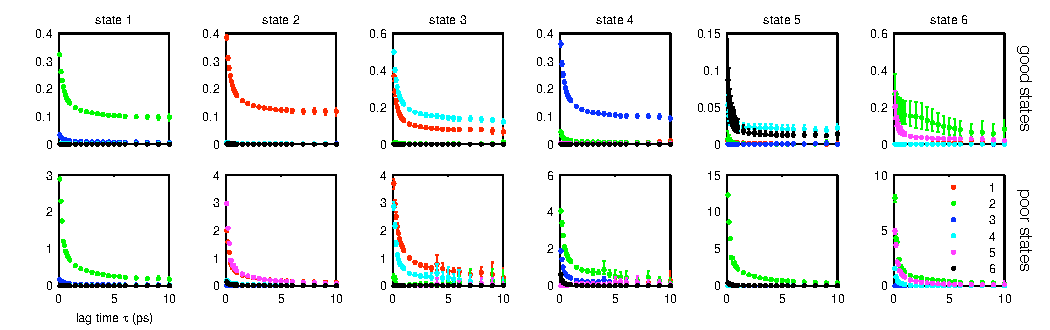
\includegraphics{chapters/mastereqn-alanine-validation/figures/implied-rates-good-and-bad.pdf}}
  \end{center}
  \caption{
  {\bf Implied transition rates as a function of lag time.}  
  For each state, the implied transition rates to all other states are shown.
  Top: Rate matrix elements implied by the observed transition matrix as a function of lag time for the ``good'' state decomposition.
  Bottom: Rate matrix elements implied by the observed transition matrix as a function of lag time for the ``poor'' state decomposition.
  }
  \label{validation:figure:implied-rates}
\end{figure*}

If the state-to-state dynamics appears Markovian after a time $\tau_{\mathrm{int}}$, we expect the relationship
\begin{equation}
\bfm{T}(\tau) = e^{\bfm{K} \tau} \:\:\forall \:\: \tau \ge \tau_{\mathrm{int}} \label{validation:equation:relation-between-transition-and-rate-matrix}
\end{equation}
where $\bfm{T}(\tau)$ is the observed transition matrix, will hold (neglecting statistical uncertainty).

At short lag times $\tau$, it is known that rate estimates will be too fast; 
in the limit where $\tau \rightarrow 0^+$, we have the same problem as in transition state theory where the neglect of recrossings results in the rate estimate to exceed the phenomenological rate constant \cite{chandler:1978a}.  
As the lag time increases beyond the time required for the system to equilibrate within the states, the longest of which is termed the \emph{internal equilibration time}, the implied rates will eventually stabilize \cite{chodera:jcp:2006}.  
However, given an arbitrary coarse-graining, the internal equilibration time may actually exceed the fast timescales in the system. 
In fact, in particularly poor choices for states, the internal equilibration time may exceed the longest timescales in the system, rendering the model useless in describing the time-evolution of the system \cite{swope:2004a}.

%Note that, even though two states may not share a common boundary in configuration space, there may still be nonzero transition rates connecting the two states at this lag time \cite{voter:1985a}.

This suggests that a way to determine $\tau_{\mathrm{int}}$ may be to compute the rate matrix $\bfm{K}$ implied by the observed transition matrix $\bfm{T}(\tau)$ for every lag time $\tau$, and identify the smallest $\tau$ after which the implied $\bfm{K}$ appears to be invariant.
At some sufficient lag time $\tau_\mathrm{eq}$, however, these rates should stabilize and a Markov description will be appropriate for all times $t$ larger than $\tau_\mathrm{eq}$ \cite{swope:2004a}.  
It is hoped that this time will be short compared to the relaxation times of the slow processes of interest in the system, such as protein folding.  

Examination of Eqs.\ \ref{validation:equation:relation-between-eigenvalues-of-transition-and-rate-matrix} and \ref{validation:equation:eigenvector-expansion-of-transition-matrix}, shows that the rate matrix can be computed from a transition matrix $\bfm{T}(\tau)$ that satisfies detailed balance by
\begin{eqnarray}
\bfm{K} &=& \bfm{U} (\tau^{-1} \log \bfm{M}) \bfm{U}^{-1} \label{validation:equation:implied-rate-matrix}
\end{eqnarray}
where $\bfm{U}$ is the matrix of eigenvectors of $\bfm{T}(\tau)$ and $\bfm{M}$ the diagonal matrix of eigenvalues.
Unfortunately, due to statistical uncertainty in the observed transition matrix $\bfm{T}(\tau)$, two things may occur that result in a rate matrix that does not satisfy the conditions enumerated in Section \ref{validation:section:master-equation-review}:
(1) some of the rates $K_{ji}, \: j \ne i$ may be negative;
(2) some of the eigenvalues of the observed transition matrix $\mu_k$ may be negative.
As a result of (2), some elements of the resulting rate matrix are complex; here, we only consider the real part.
To ensure that the conditions of nonnegativity and reality of rates are met, one may use more sophisticated methods to recover rate matrices that only approximately satisfy Eq.\ \ref{validation:equation:relation-between-transition-and-rate-matrix} yet satisfy these conditions \cite{grubmueller:1994a,sriraman:2005a}.

We computed the implied rate matrix as a function of lag time from the observed transition matrices using Eq.\ \ref{validation:equation:implied-rate-matrix} for the 10 ps shooting trajectories.
The implied rates for good and poor partitionings are shown in Figure \ref{validation:figure:implied-rates}.
As expected, the rates approach their transition state theory estimates as the lag time $\tau$ approaches zero and decay as the lag time increases.
For the good state decomposition, the rates appear to approach a constant value (to within statistical uncertainty) at lag times around 6 ps.
State 6 is clearly the most problematic, with the uncertainties for transition to state 4 being especially large and only converging to a constant value very late.
This may suggest that this state in particular could benefit from refinement of the state boundaries.
The poor decomposition has much faster rates, consistent with a model with shorter aggregate timescales.
It is not evident if the rates converge over 10 ps --- they appear to be still diminishing near lag times of 10 ps, though at a slow rate.
% JDC: Do we have to blow these up, or plot on a log scale?
% JDC: Should we also show lumped?

\subsection{Eigenvalues of the implied rate matrix.}
\label{validation:section:timescales-test}

\begin{figure}[tbp]
  \begin{center}
    \resizebox{3.375in}{!}{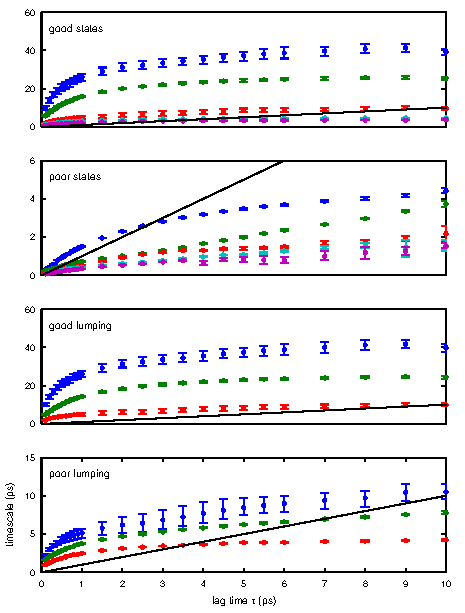
\includegraphics{chapters/mastereqn-alanine-validation/figures/timescales.pdf}}
  \end{center}
  \caption{
  {\bf Implied timescales of the rate matrix as a function of lag time.}  
  Implied timescales and associated uncertainties are shown for good decomposition (top), poor decomposition (middle upper), good lumping (middle lower), and poor lumping (lower).
  Timescales are colored by order from longest (blue) to shortest (purple).
  The black line denotes $\tau_k = \tau$, such that processes whose timescales fall below this line occur on times shorter than the lag time.
  }
  \label{validation:figure:timescales}
\end{figure}

%\begin{itemize}
%\item If the model holds for some coarse-grained time, we expect $\bfm{T}(\tau) = e^{\bfm{K} \tau}$ for all $\tau > \tau_\mathrm{eq}$.
%\item We could determine the individual rate matrix elements from each transition matrix $\bfm{T}(\tau)$ at different $\tau$, but we might instead examine the eigenvalues of the rate matrix $\bfm{K}$, which also give information about the \emph{aggregate timescales} of processes that $\bfm{K}$ describes.
%\item Aggregate processes are related to phenomenological (observed) kinetics --- in a two-state model, the phenomenological rate would be the sum of forward and backward rates.
%\item Instead of plotting rates, we can plot the slowest timescales (inverse rates) associated with the system.
%\item These timescales are also easier to extract from noisy transition matrices.  If transition matrix satisfies detailed balance, the eigenvalues will at least be real, though some may be negative, causing problems with inferring \bfm{K}.
%\item Some eigenvalues of the transition matrix might die out (approach zero) at some $\tau$, in which case the numerical and statistical noise will cause them to remain slightly above zero and cause the perceived timescales to grow at a linear rate.
%\end{itemize}

As the number of states, $N$, increases, the number of rate matrix elements increases as $N^2$.
Examination of all of these for signs of convergence may be impractical.
Additionally, we are generally concerned with only the \emph{slowest} processes in the system.
Note that the time evolution of an observable $A(\q)$ can be written in terms of the eigenvector expansion (Eq.\ \ref{validation:equation:eigenvector-expansion-of-transition-matrix}) as
\begin{eqnarray}
\expect{A}(t) &=& \sum_{k=1}^N (\bfm{A}^\T \bfm{D}^{1/2} \tilde{\bfm{u}}_k) \, (\tilde{\bfm{u}}_k \bfm{D}^{1/2} \bfm{p}(0)) \, e^{\lambda_k t} \nonumber \\
&=& \sum_{k=1}^N c_k \, e^{-t / \tau_k}
\end{eqnarray}
where $\bfm{A}$ is the vector of characteristic spectroscopic observables over each individual state, $\tau_k$ is a characteristic timescale for the process governed by eigenvector $\bfm{u}_k$, and $c_k$ is its (potentially negative) amplitude.
It may be that some non-Markovity is tolerated if it only disrupts the fastest processes in the system but leaves the slowest ones, which may serve to determine the behavior of $\expect{A}(t)$ over the timescales of interest, unaffected.
In fact, if the model is only Markovian on timescales greater than $\tau_\mathrm{int}$, processes with characteristic timescales $\tau_k < \tau_\mathrm{int}$ will not correctly be described by the model anyway.
Additionally, because we only extract $N-1$ values from the transition matrix instead of $N^2$, these values may be better determined statistically than the individual rates.
% JDC: Is this true?  can we include some sensitivity analysis?

As a result, Swope \emph{et al.}\ \cite{swope:2004a} suggested that the implied timescales of the rate matrix, computed from the observed transition matrix as a function of lag time, could be used to determine the onset of Markovian behavior.
These timescales are determined from the eigenvalues $\lambda_k$ of the rate matrix, which can in turn be determined directly from the eigenvalues of the transition matrix through Eq.\ \ref{validation:equation:relation-between-eigenvalues-of-transition-and-rate-matrix}:
\begin{eqnarray}
\tau_k = - \lambda_k^{-1} = - \tau [\log \mu_k]^{-1} \:\:,\:\: k = 2,\ldots,N
\end{eqnarray}
If the elements of the implied rate matrix converge to some fixed value for lag times $\tau \ge \tau_\mathrm{int}$, then these implied timescales will also converge.
While the converse is not true, we may be unlikely to encounter a case where the timescales have converged but many of the individual rates are still changing significantly.

We computed the timescales as a function of lag time for the 10 ps shooting trajectories for all four state decompositions, and depicted in Figure \ref{validation:figure:timescales}.
The timescales of the good state decomposition all appear to fluctuate about a constant value (to within statistical uncertainty) at lag times of 6 ps or greater, where three of the timescales are larger than the lag time at this point.
By contrast, the slowest timescales for the poor decomposition do not appear to stabilize within 6 ps, and all processes appear \emph{faster} than the lag time after lag times of 3 ps.
The good lumping does not appear to disrupt the longest timescales --- three timescales greater than the lag time are again observed at a lag time of 6 ps.
The poor lumping,  on the other hand, diminished the timescales such that by 9 ps, when it appears the timescales \emph{may} have reached a plateau, only one timescale is barely longer than the lag time.

%\subsection{Transition probabilities}
%\label{validation:section:transition-probabilities}

%\begin{itemize}
%\item If the model accurately describes dynamics, it should be able to reproduce state-to-state correlation functions (or transition probabilities or state occupation probabilities) over times longer than $\tau_{\mathrm{int}}$.
%\item Unfortunately, the trajectories are rather short, so the maximum $n$ for which $n \tau \le T$ may be small or even 1.
%\item For every lag time, we could conceivably compute the predicted transition probabilities and compare to the observed transition probabilities to assess agreement, but it is not clear how to quantify deviation because of the correlation in uncertainties between successive lag times.
%\end{itemize}

\subsection{Second-order transition probabilities.}
\label{validation:section:second-order-transition-probabilities}

\begin{figure*}[tbp]
  \begin{center}
    \resizebox{\textwidth}{!}{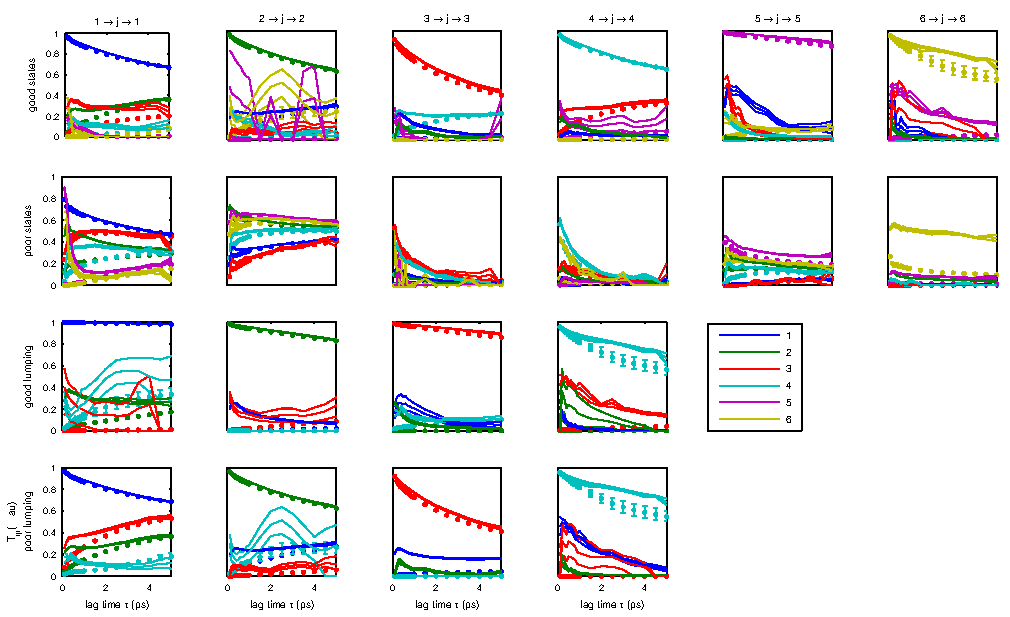
\includegraphics{chapters/mastereqn-alanine-validation/figures/second-order-transition-probabilities.pdf}}
  \end{center}
  \caption{
  {\bf Second-order transition probabilities compared with products of first-order transition probabilities as a function of lag time.}  
  Observed second-order transition probabilities $T_{k|ji}(\tau)$ are shown as solid lines with the envelope indicating a 68\% confidence interval, while first-order transition probabilities are shown as points with error bars.
  Because there are $6^3 = 216$ second-order transition probabilities, and many of them are not well estimated by the limited dataset, only the 36 $T_{i|ji}(\tau)$ transition probabilities are shown.
  Each plot shows 6 transition probabilities originating from a single state $i$, occupying a state $j$ at time $\tau$, and returning to $i$ at time $2\tau$.
  }
  \label{validation:figure:second-order-transition-probabiliites}
\end{figure*}

A more direct test for the effects of history dependence is the examination of second-order transition probabilities $T_{k|ji}(\tau)$, which denotes the probability of observing the system in state $k$ at time $2\tau$ given that it was initially in $j$ at time $\tau$ and $i$ at time $0$ \cite{swope:2004a}.
These transition probabilities can be estimated from three-time correlation functions $C_{kji}(\tau) = \expect{\chi_k(2\tau) \chi_j(\tau) \chi_i(0)}$ by
\begin{eqnarray}
T_{k|ji}(\tau) &=& \frac{C_{kji}(\tau)}{\sum\limits_{k'=1}^M C_{k'ji}(\tau)} . \label{validation:equation:second-order-transition-matrix}
\end{eqnarray}
If the Markovian property holds at lag time $\tau$, the probability of observing a transition from state $j$ to state $k$ should be independent of the previous state $i$:
\begin{eqnarray}
T_{k|ji}(\tau) = T_{kj}(\tau) \:\:\forall\:\: \tau \ge \tau_\mathrm{int} .
\end{eqnarray}
Ideally, we would verify that all observed second-order transition probabilities are equal to the corresponding first-order transition probabilities to within statistical uncertainty.

Second-order transition matrices were computed from correlation functions $C_{kji}(\tau)$ estimated from the shooting data using Eq.\ \ref{validation:equation:second-order-transition-matrix} above, and these are shown in Figure \ref{validation:figure:second-order-transition-probabiliites} together with their corresponding first-order transition probabilities estimated from the same dataset.
Because there are $N^3 = 216$ possible three-time correlation functions, and because the observed data for transitions where $i \ne j \ne k$ will be sparse, we choose to only examine those where $k = i$. 
One obvious limitation of this approach is the requirement that the trajectories be at least $2\tau$ in length, so we are not even able to reach the 6 ps lag time required for Markovianity.
It is also evident that there is a large amount of statistical uncertainty in the resulting second-order transition matrix, so much so that it is difficult to discern whether disagreement is meaningful, as in the $2\rightarrow j\rightarrow 2$ plot for the good partitioning.

\subsection{Chapman-Kolmogorov equation.}
\label{validation:section:chapman-kolmogorov-test}

\begin{figure*}[tbp]
  \begin{center}
    \resizebox{\textwidth}{!}{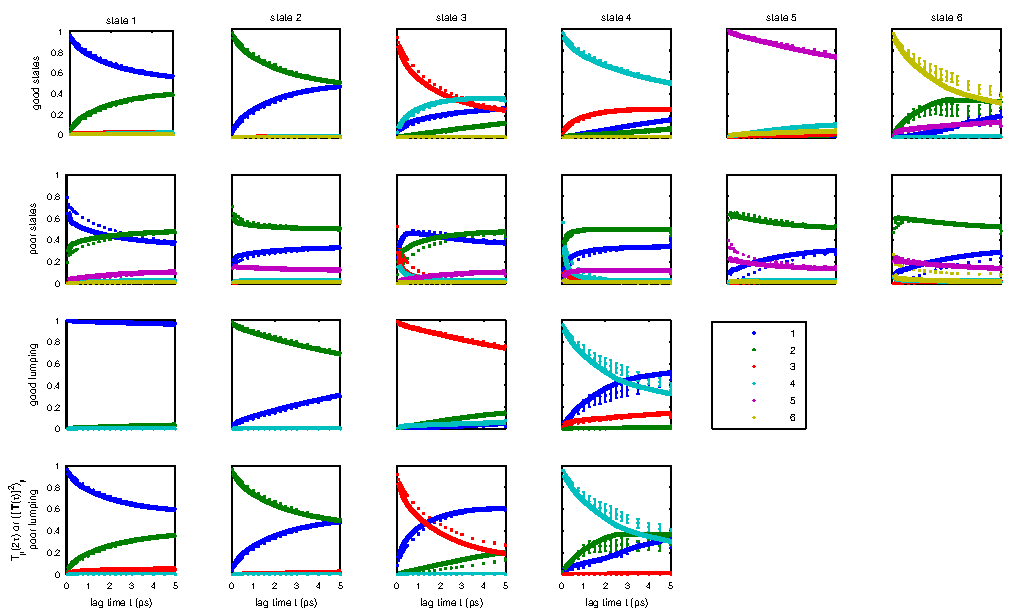
\includegraphics{chapters/mastereqn-alanine-validation/figures/chapman-kolmogorov.pdf}}
  \end{center}
  \caption{
  {\bf Test of the Chapman-Kolmorov equation.}  
  Observed transition probabilities $T_{ji}(2\tau)$ are shown as points with error bars, while predicted transition probabilities from $([\bfm{T}(\tau)]^2)_{ji}$ are shown as lines enveloping a 68\% confidence interval.
  }
  \label{validation:figure:chapman-kolmogorov}
\end{figure*}

Due to the large statistical uncertainty in the three-time correlation functions $C_{kji}(\tau)$ used to compute the second-order transition probabilities, and the $N^3$-dependence of $T_{k|ji}(\tau)$ on the number of cells, it may be useful to instead consider whether the Chapman-Kolmogorov equation is satisfied at some minimum $\tau$:
\begin{eqnarray}
\bfm{T}(2\tau) &=& [\bfm{T}(\tau)]^2 \label{validation:equation:chapman-kolmogorov}
\end{eqnarray}
Here, only $N^2$ elements need be compared, and intermediate states are effectively ummed over.
Figure \ref{validation:figure:chapman-kolmogorov} shows a comparison of the left-hand side and right-hand side estimated independently from the 10 ps shooting trajectories.
It is again apparent that this metric, too, requires trajectories of minimal length $2\tau$ to test the satisfaction of Eq.\ \ref{validation:equation:chapman-kolmogorov} for a lag time of $\tau$.
Somewhat surprising is the observation that, for the good partitioning, the Chapman-Kolmogorov property appears to be satisfied within statistical uncertainty at very \emph{early} times, up to perhaps 1 ps.
This is counterintuitive, as it is clear that models constructed from such short lag times poorly reproduce dynamics \cite{chodera:mms:2006}.
It is hard to determine whether the condition is satisfied at longer times, as state 6 appears particularly problematic in the good decomposition.
Surprisingly, the poor decomposition does not appear much worse than the good decomposition over the span of times considered, though the poor lumping shows more systematic deviation than the good lumping throughout lumped state 3.

\subsection{Discrete lifetime distribution.}
\label{validation:section:lifetime-distribution-test}

\begin{figure*}[tbp]
  \begin{center}
    \resizebox{\textwidth}{!}{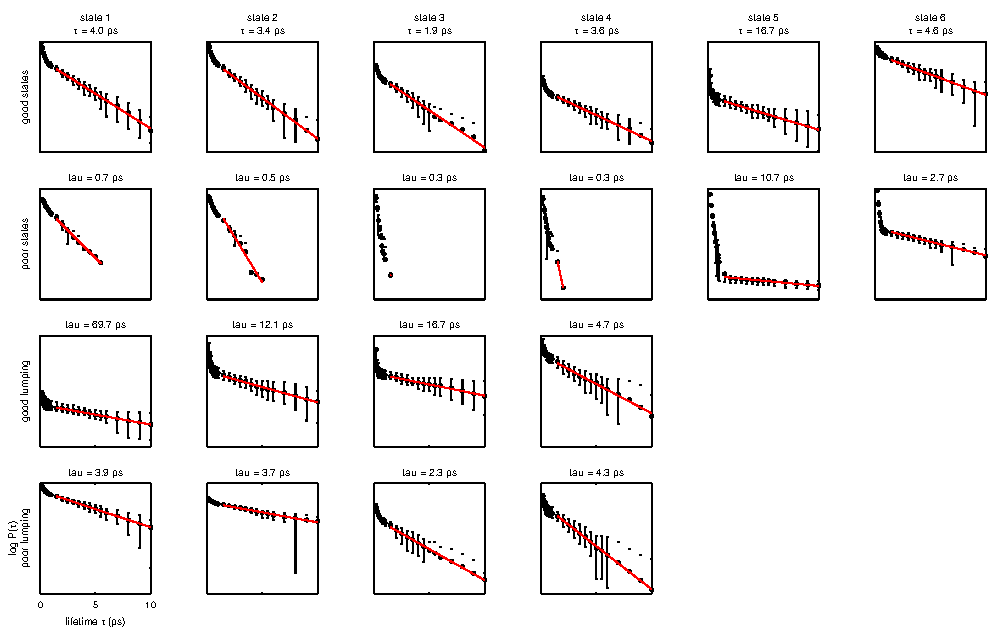
\includegraphics{chapters/mastereqn-alanine-validation/figures/discrete-lifetimes.pdf}}
  \end{center}
  \caption{
  {\bf Observed and geometric discrete lifetime probability distributions.} 
  The logarithm of the discrete lifetime probability mass function $P(L ; \tau)$ for each state, which indicate the probability of observing the system to remain within a given state for exactly a a number  of consecutive observation intervals $L$, is shown as a function of $L \tau$ along with the characteristic lifetimes obtained from a linear fit to the log probability over the interval $L \tau \in [1.5,10]$ ps, evaluated with sampling interval $\tau_\mathrm{sample}$ = 0.1 ps.
  The number of intervals $L$ for which the system remains in one state has been multiplied by the sampling interval $\tau$ so that the x-axis appears in units of time.
  Top: good states; middle top: poor states; middle bottom: good lumping; bottom: poor lumping.
  }
  \label{validation:figure:lifetime-distributions}
\end{figure*}
% JDC: We should probably be generating these plots for many different tau, and trying to find the tau for which they all appear to be linear.

For a discrete- or continuous-time master equation model, if the system is initially in state $i$ at time $t=0$, the probability that it will be observed to remain in state $i$ for exactly $L-1$ additional consecutive observations with observation interval $\tau$ is given by the geometric distribution \cite{swope:2004a}, with probability mass function
\begin{eqnarray}
P(L ; \tau) &=& (1 - T_{ii}(\tau)) [T_{ii}(\tau)]^{L-1} \:, L \in \{1, 2, \ldots, \} . \label{validation:equation:lifetime-distribution-pmf}
\end{eqnarray}
and cumulative distribution function
\begin{eqnarray}
P(L \le K; \tau) &=& 1 - [T_{ii}(\tau)]^K .		
\end{eqnarray}
When $\log P(L ; \tau)$ is plotted as a function of $L$ for fixed lag time $\tau$, the trend should be linear for $\tau \ge \tau_\mathrm{eq}$ with slope $\log T_{ii}(\tau)$, though its behavior may differ at short times before Markovianity has been achieved.

%The master equation prescribes first-order interstate transition kinetics, and so the probability of the system remaining in some state $i$ for a time $t$ before leaving, the lifetime of $i$, should be given by the exponential distribution:
%\begin{eqnarray}
%p_i(t) \, dt = - k_{ii} \, e^{-k_{ii} t} \, dt
%\end{eqnarray}
%Because data collected from the molecular dynamics simulations is sampled at discrete intervals, we cannot compute the true lifetime probability density function $p_i(t) \, dt$.  Instead, we consider the discrete lifetime distribution $p_i(n)$, which is the probability that the system spends $n$ intervals of time $\Delta t$ in state $i$.  The probability mass function $p_i(n)$ is given by
%\begin{eqnarray}
%p_i(n) &=& \left< L_n[\bfm{z}(t)] \right> \\
%&=& \frac{\mathcal{D}[\bfm{z}(t)] \, \mathcal{P}[\bfm{z}(t)] \, L_n[\bfm{z}(t)]}{\mathcal{D}[\bfm{z}(t)] \, \mathcal{P}[\bfm{z}(t)]}
%\end{eqnarray}
%Note that $p_i(n)$ is normalized such that $\sum_{n=0}^\infty p_i(n) = 1$.

%\emph{JDC: WE ACTUALLY COMPUTE PRODUCT OF ONE-TIME $i \rightarrow i$ TRANSITION PROBABILITIES.} Because the system is only observed at discrete intervals in time, the lifetime observed is not a true lifetime, but rather the number of consecutive observations where the system remains in the same state; the system may have indeed left the state and returned in between observations, but this cannot be known.  If we denote the probability of observing $m$ consecutive observations in state $i$ by $P_{im}$, we can compute this from the true transition matrix by
%\begin{eqnarray}
%P_m = T_{ii}^m = \left( e^{\bfm{K} \tau} \right)_{ii}^m
%\end{eqnarray}
%(Normalization?  Is this a CMF or a PMF?)

%The observed probability of $m$ consecutive observations is
%\begin{eqnarray}
%\hat{P}_m = \sum_{k=1}^K w_k \frac{1}{N T} \sum_{n=1}^N \sum_{t=1}^{T-m} \chi_i(\bfm{z}_{knt}) \chi_i(\bfm{z}_{kn(t+1)}) \cdots \chi_i(\bfm{z}_kn(t+m))
%\end{eqnarray}

Figure \ref{validation:figure:lifetime-distributions} shows the observed $\log P(L;\tau_\mathrm{sample})$ for each state, determined by constructing a histogram of the number of successive snapshots the system is observed to remain in state $i$, along with the geometric distribution with the same mean lifetime.  
At large $L$, all states show geometric lifetime distributions, but at short times, more complex behavior is observed.
States 5 and 6 of the good manual decomposition, for example, appear to exhibit two distinct geometric phases.
In all cases, the onset of the final linear behavior is very early --- within enough sampling intervals such that the remainder of the plot is linear for $L \tau_\mathrm{sample} > 2$ ps.
This is, of course, too early for the onset of Markovian prediction.
It is possible that examination of the complete set of plots for various sampling intervals $\tau$ would allow one to better estimate the onset of Markovian behavior, but this may be difficult, as the number of these grows as $N T / \tau_[\mathrm{sample}$t.

%In state 5, the jagged features of the observed lifetime distribution suggests transitions out of this state may still be insufficiently sampled.  

% JDC: Check if few trajectories dominate estimate.
% JDC: Which tau(s) to use? 


%\subsection{Assessment of Markovian behavior.}

%In order for a transition matrix or rate matrix to be of use in describing the time-evolution of the system probabilities or the dynamics of a single trajectory through the system, several properties must hold.  First, the lag time $\tau$ must be large enough for the process to be memoryless; that is,
%\begin{equation}
%P(i, j, k) = P(k | j) P(j | i) P(i)
%\end{equation}

%\subsubsection{Eigenvectors.}
%\label{validation:section:eigenvectors}

%\begin{figure}[tbp]
%  \begin{center}
%    \resizebox{3.375in}{!}{\includegraphics{figures/shoot-100ps:eigenvectors.pdf}}
%  \end{center}
%  \caption{\bfm{Eigenvectors of the transition matrix as a function of lag time.} Left: left eigenvectors.  Right: right eigenvectors.} \label{validation:figure:shoot-100ps:eigenvectors-vs-lag-time}
%\end{figure}

%\begin{figure}[tbp]
%  \begin{center}
%    \resizebox{3.375in}{!}{\includegraphics{figures/ev-K.pdf}}
%  \end{center}
%  \caption{\bfm{Left eigenvectors of the rate matrix show hierarchical state structure.}  For each eigenvector, each state is colored according to the sign and magnitude of its eigenvector component: blue (negative) to red (positive).  States colored similarly have similar values for their eigenvector component.  It is readily apparent that, at fast timescales, that states 1 and 2 (which are separated by a relatively small barrier) are uncoupled, whereas at longer timescales they act like a single, larger state.}
%  \label{validation:figure:hierarchy}
%\end{figure}

%%%%%%%%%%%%%%%%%%%%%%%%%%%%%%%%%%%%%%%%%%%%%%%%%%%%%%%%%%%%%%%%%%%%%%%%%%%%%%%%%%%%%%%%%%%%%%%%%%%%%%
% DISCUSSION AND CONCLUSIONS
%%%%%%%%%%%%%%%%%%%%%%%%%%%%%%%%%%%%%%%%%%%%%%%%%%%%%%%%%%%%%%%%%%%%%%%%%%%%%%%%%%%%%%%%%%%%%%%%%%%%%%
\section{Discussion and Conclusions}

% Outline:
% - We have presented an evaluation of a number of methods for determining, given a state decomposition, what lag time a master equation model constructed from simulation data will accurately reproduce long-time dynamics, provided this time is shorter than the trajectories used to construct the model.
% - As the internal equilibration time cannot yet be computed directly, our tests evaluate whether a number of consequences of Markovian behavior hold.

Here, we have examined the issue of how one may verify whether a Markov chain or master equation model constructed from a set of short trajectories will be able to reproduce dynamics over long times without necessitating comparison with a separate set of long trajectories.
Due to the difficulty of computing the internal equilibration time $\tau_{\mathrm{int}}$, the time required for the system to lose memory within the states, we considered a number of tests of Markovianity based on determining whether conditions corresponding to consequences of Markovian behavior were satisfied to within our ability to resolve by statistical uncertainty.
Not all of these tests were of equal utility.
Some tests, such as comparison of second-order transition probabilities with first-order transition probabilities, were too noisy to provide useful information directly.
Summation over intermediate states to give a test of the Chapman-Kolmogorov equation reduced the statistical uncertainty, but this condition was met to within statistical uncertainty at lag times that were too short to accurately reproduce dynamics.
Examination of discrete lifetime distributions revealed clear non-Markovian behavior at short times, but this test too gave indication that Markovian behavior was achieved at lag times that were too short.
Examination of the implied rate matrix elements or timescales was informative of the time of emergence of Markovian behavior, but as the number of rate matrix elements increases as $N^2$, and some non-Markovitianity might be tolerated if the slowest processes are preserved, examination of the slowest timescales was deemed the most useful of these metrics for verifying Markov behavior.

Many challenges to efficiently constructing useful master equation or Markov models of protein dynamics remain.
The selection of an appropriate state space, a topic addressed in Ref.\ \cite{chodera:jcp:2006}, is perhaps the most difficult of these.
Even given an optimal decomposition into a desired number of states for a desired number of states, whether the timescale on which this model becomes Markovian is accessible and the quantity of simulation data needed to construct accurate models is not know.
Additionally, efficient methods for computing interstate transition rates are needed.
The success of these models in accurately describing the dynamics of small solvated peptides is encouraging, but their utility in characterizing complex biomolecular dynamics of large macromolecules remains to be seen.

%%%%%%%%%%%%%%%%%%%%%%%%%%%%%%%%%%%%%%%%%%%%%%%%%%%%%%%%%%%%%%%%%%%%%%%%%%%%%%%%%%%%%%%%%%%%%%%%%%%%%%
% ACKNOWLEDGMENTS
%%%%%%%%%%%%%%%%%%%%%%%%%%%%%%%%%%%%%%%%%%%%%%%%%%%%%%%%%%%%%%%%%%%%%%%%%%%%%%%%%%%%%%%%%%%%%%%%%%%%%%
\section{Acknowledgements}

The authors happily thank Nina Singhal, Sanghyun Park, Vijay Pande, and Hans Andersen (Stanford) for many enlightening discussions, and Libusha Kelly (UCSF) for critical comments on this manuscript.
JDC was supported by Howard Hughes Medical Institute and IBM predoctoral fellowships.  
WS acknowledges support from NSF MRSEC Center on Polymer Interfaces and Macromolecular Assemblies DMR -- 0213618, and KD the support of NIH grant GM34993. 

%%%%%%%%%%%%%%%%%%%%%%%%%%%%%%%%%%%%%%%%%%%%%%%%%%%%%%%%%%%%%%%%%%%%%%%%%%%%%%%%%%%%%%%%%%%%%%%%%%%%%%
%\bibliographystyle{jdc} 
%\bibliography{mastereqn-alanine-validation}

%\end{document}
